\section{Planning \& Group-Work Approach}

\subsection{Development of a Plan}

During the first couple of weeks of the project the group members formed into a
working team,
and after receiving a detailed brief from the customer via video-call quickly
went about setting up ground rules about how the project should be executed. It
was decided that weekly meetings with the project supervisor would be
appropriate, with one to two more group meetings during each week, as required.
It was decided that meetings should be informal in general, with rough minutes
taken in a log book for future reference, to try and cut down on any unnecessary
 overhead.

%TODO: link to appendix using latex foo
The group established an understanding of the task, and created a project
brief in response to the first customer meeting. This contained a rough overview
of the group's understanding of the task, and can be found attached in appendix
A. The Gantt chart in the project brief is an elaboration on a project lifecycle
shown in Figure \ref{fig:l1plan-1}, chosen to fit in with the two customer
presentations over the course of the project so that a presentable work package
could be shown to the customer at each milestone. This approach also gives as
much room as possible
for using agile methods in the underlying development approach (discussed in
more detail below). Further discussion of the time management
methods used by the group, with a more detailed evaluation of the Gantt charts
produced over the course of the project can be found in the evaluation section
of this report.

\begin{figure}[htb]
\centering
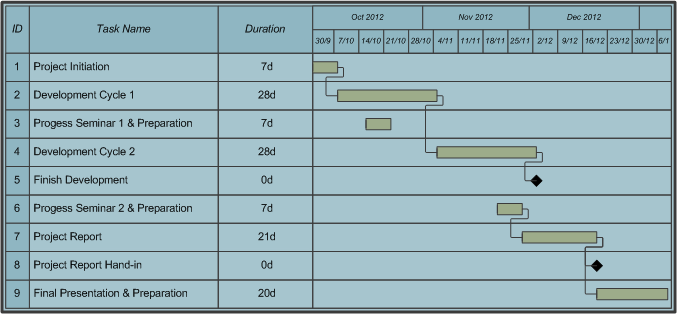
\includegraphics[width=0.8\textwidth]{img/l1plan.png}
\caption{Level 1 Plan}
\label{fig:l1plan-1}
\end{figure}


Once the group had established an initial breakdown of the tasks involved with the
project and a general idea of the approaches the group could take,
 a skills audit was held to discuss which team members were best
qualified for the various roles required by the project. The table below shows
a summary of the audit including the skills relevant to the approach taken.

\begin{center}
%\begin{table}
\begin{tabularx}{\linewidth}{|XXX|}
\hline
Group Member & Skill & Level of Expertise (1-5) \\ \hline
Thomas Grainger & Python & 5 \\
& Python Frameworks & 3 \\
& Distributed Sytems & 4 \\ \hline
Weike Liao & Python & 3 \\
& Distributed Systems & 4 \\ \hline
Chris Orchard & Python & 4 \\
& Project Management & 3 \\
& Systems Integration & 5 \\ \hline
Nafiseh Vahabi & AI & 5 \\
& Python & 4 \\
\hline
\end{tabularx}
%\end{table}
\end{center}

%maybe more stuff about streams of work?
After some background research had been performed, the group decided to split
the development tasks into discrete components allowing members of the group to
work in the areas of most experience, using their specialist understanding of a
given area to research and develop in an automomous fashion with progress and
code produced periodically reviewed by the other members of the group. The
individual streams of work should meet at the customer milestones to allow some
integration testing and to present some new working functionality to the
customer.

\subsection{Group-work Approach}
%TODO: elaborate to an appropriate extent
The development approach used for the project draws inspiration from agile
methods, with two
development iterations over the 10 week life of the project. Whilst ideally more
iterations would be made, allowing more customer involvement, the
structure and timescale of the project meant that this was not possible. If
there had been more available development time, the project would have defined
phases for the inception and elaboration of the project following a Unified
Process approach (CITE), instead the inception and elaboration tasks are
interleaved into the first development iteration as shown on the Gantt charts. 

At the time of the skills audit, the group also investigated appropriate tooling
for the development to be carried out. The programming language chosen to implement the
solution in was python, as all of the group members had some experience
with the language, and it was also noted that python code was generally easier to
read than some of the other options available, making code review somewhat
easier. Another advantage of choosing python was the inclusive developer
community, allowing the group to contribute a bug fix back to one of
the tools used by the project, utilising some prior experience in python distributed
frameworks.
For version control, git was chosen as most of the group had previous experience
with the tool, and the group also chose to use GitHub to host the code
repository (in a private repository) removing some risks associated with the
possibility of ECS systems failure. GitHub gave the group an easy way to monitor
commits and view the diff made by any given commit, a feature that made the
process of reviewing committed code much quicker. GitHub also presents a
RESTful API that the group
found useful for developing metrics tools. This report is written in LaTeX,
mainly to ease the burden of version control and collaborative editing by using
multiple files, but also to enable metrics to be generated for report progress
during the write up.

%adjust to say less not-production-ready?
Choosing and enforcing an appropriate level of quality control for the code
developed was an important task throughout the project. The customer specified
that they would prefer a solution along the lines of a high-fidelity prototype,
as a way of achieving a maximal amount of useful work, with further testing to transition
to a production-ready system if the developed product proved to be useful
(outside of the scope of the project). This
is not to say that the code was not tested and reviewed throughout the project,
just that testing and review were not enforced as vigorously as might be
required for direct production use.

%example of use cases, use cases??!
At a very early stage of the project, the use of a distributed task framework as
a platform for the project was considered the preferred way to construct the
project, and this design decision was made for a variety of technical reasons
detailed in the technical approach section of this report. There are also some
benefits for managing the development effort from using such a framework. The
framework allows each component to be developed in relative isolation from the
other components, with low coupling between the different parts of the system.
This also served as a method for mitigating some of the risks associated with
individual components in the system either not working, or not being suitable
for a given use case when deployed by the customer.

During the development of the project, the group had to make two presentations
detailing the progress made up to that point, addressed to the supervisor,
customer, and a selection of peers. The Level 1 plan above shows the gaps left
for the preparation of each presentation. For each presentation, the group first
came up with an appropriate structure for the presentation, and then constructed
the relevant slides according to which parts of the work being presented each
member of the group was responsible for. An equivalent process will be used for
the final end-of-project presentation.


\subsection{Risk Management}

As part of the project management task, possible risks associated with the
project were identified, and steps taken to mitigate them. The risks identified
by this process are listed in the table below. Throughout  the
project, precedence was given to tasks with outstanding risk, or risks that had
not been assessed, as a means of minimising the risk of the project not being
finished by the deadline.

\clearpage
\begin{landscape}
%\thispagestyle{empty}
%\makebox[\textwidth]{
\small
\setlength\LTleft{0pt}
\setlength\LTright{0pt}
\begin{longtable}{@{\extracolsep{\fill}}|p{5cm}p{1cm}p{2cm}p{6cm}p{2cm}p{2cm}l|}
    %\begin{tabularx}{1.5\textwidth}{|p{5cm}XXp{5cm}XXl|}
        \hline
        Risk & Impact (1-5) & Probability (1-5) & Mitigation & Risk Score (1-25) & Mitigated Risk Score & Status \\ \hline
        The delivered project does not meet the provided specification. & 5 & 2 & Ensure that progress is monitored throughout the project and that any necessary change in specification is discussed with the customer. & 10 & 8 & Not Impacted \\
        \hline 
        The delivered project does not meet customer expectations & 5 & 2 & Ensure customer is aware of the status of the project and likely outcome throughout the course of the project lifecycle & 10 & 4 & Mitigated \\ 
        \hline
        A tool or library chosen for use in the development of the project does not meet its requirements. & 4 & 3 & Chose tools and libraries that group members are familiar with, and preferably those which can be patched by group members where possible. & 12 & 6 & Mitigated \\ 
        \hline
        Integration takes much longer than planned due to conflicting styles of coding in software components developed be different group members & 3 & 4 & Discuss and enforce a single style of coding for all software, reviewing code as it is written. & 12 & 3 & Mitigated \\
        \hline
        The code contributed by a team member does not perform as expected or is not completed to the necessary quality & 4 & 2 & Review all code committed to the source repository, use pair coding if possible. & 8 & 4 & Not Impacted\\
        \hline
        A group member struggles with a task due to not having the necessary skills to perform the task & 4 & 2 & Use a skills audit to determine the confidence of the group members in various tasks, and allocate work accordingly. Monitor progress throughout the project and re-allocate work if necessesary & 8 & 4 & Mitigated \\
        \hline
        Interaction with the customer leads to a significant expansion of scope of the project, causing the project not to be delivered on time. & 5 & 2 & Be vigilant of any possible scope creep, and discuss the implementation time of any requested changes with the customer. & 10 & 6 & Not Impacted\\ 
        \hline
        Infrastructure hosting critical parts of the project such as the source code repository suffer from a critical failure, preventing access or causing loss of work. & 5 & 2 & Use a distributed version control system such as git for all code and written documentation, hosted on a large reputable code hosting service such as GitHub.  & 10 & 2 & Mitigated\\
        \hline
        A member of the team falls ill, preventing them from contributing significantly to a given part of the project. & 5 & 2 & Ensure a low "bus factor" is maintained, and that no single group member is given responsibility for a larger than necessary portion of critical tasks. & 10 & 8 & Not Impacted\\
        \hline
        The group is not given the necessary permissions from iSolutions and JANET to operate the project on university systems. & 4 & 3 & Communicate the intent and reasoning for the project at an early stage, ensure suitable preventative measures are implemented to prevent adverse effects from the malware scanning component of the project. If possible, keep a group member's personal computer as a contingency. & 12 & 6 & Mitigated\\
        \hline
        ECS are not able to provide the group with the resources necessary to run the project. & 4 & 1 & Request sufficient resources at an early stage, track the resource usage of the project during development and attempt to keep resources used during scanning to the minimum necessary & 4 & 2 & Not Impacted\\
        \hline
    %\end{tabularx}
\end{longtable}
%}
\end{landscape}
%Risk approach???

\subsection{Stakeholder Management}

%TODO:JANET explanation
%TODO:call isolutions isolutions?
%are supervisor/second supervisor stakeholders?
Although interaction with the customer has been detailed previously, there are
also some other stakeholders of note, specifically in relation to the use of the
University of Southampton's infrastructure and JANET's network link to
potentially download (and try to execute in some cases) large volumes of
malware. A solution was found to the technical challenge of how to restrict
possible malicious activity caused by malware being analysed by the system, as
discussed in the technical approach. Once the preventative technical measures
had been discussed with members of ECS systems staff and judged adequate, both
JANET and the University computing service were contacted to inform them of the
intended activity, and to invite comment. A conversation ensued with the
technical staff of the University infrastructure team, who not only felt that
the measures being taken were adequate but was a model solution of how such work
should be carried out in the future. All of the contact detailed above took
place via the groups single point of contact for the stakeholders. Although
having a single person responsible for all stakeholder contact is not risk
averse, this is offset by the advantage of the stakeholders only having to deal
with a single person, not having to link together several email addresses or
identities, and mitigating the risk of the conflicting messages being sent to a
stakeholder from different group members.

